\documentclass[11pt,a4paper]{article}
\usepackage{graphicx}
\usepackage{longtable}
\usepackage{float}
\usepackage{wrapfig}
\usepackage{rotating}
%\usepackage{a4wide}
\usepackage[normalem]{ulem}
\usepackage{amsmath}
\usepackage{textcomp}
\usepackage{marvosym}
\usepackage{wasysym}
\usepackage{amssymb}
\usepackage{hyperref}
%\usepackage[utf8]{inputenc}
%\usepackage[T1]{fontenc}
%\usepackage{polyglossia}
%\setmainlanguage[]{french}
\usepackage[top=30pt,bottom=30pt,left=48pt,right=46pt]{geometry}
\usepackage{listings}

\lstset{
    language=C++
  , frame=single
  , basicstyle=\scriptsize
  , keywordstyle=\color{blue}\bfseries
  , commentstyle=\color{red}
  , stringstyle=\color{magenta}\ttfamily
  , backgroundcolor=\color{black!5}
}

\usepackage[dvipsnames]{xcolor}
\usepackage{subfigure,tikz}
\usetikzlibrary{shadows,shadows.blur, trees,matrix,arrows,decorations}
\usetikzlibrary{decorations.pathmorphing, fadings, shapes, shapes.arrows, positioning, calc, shapes,fit}
\usepackage{fp}
\usepackage{pgfplots}
\tolerance=1000
\author{Xavier JUVIGNY}
\date{\today}
\title{Travaux dirigés n°3}

\newtheorem{definition}{Définition}
\newtheorem{theo}{Théorème}

\definecolor{verylightgray}{rgb}{0.95 0.95 1.0}

\definecolor{darkblue}{rgb}{0. 0. 0.4}

\begin{document}
\maketitle
\tableofcontents

\section{Produit scalaire}

\begin{itemize}
\item \`A partir du fichier \texttt{dotproduct.cpp}, paralléliser le calcul du produit scalaire à l'aide de directives OPENMP;
\item Calculer l'accélération du produit scalaire en faisant varier le nombre de threads à l'aide de la variable d'environnement
\texttt{OMP\_NUM\_THREADS}. Comment expliquez-vous le résultat que vous obtenez pour l'accélération ?
\item \'Ecrire une deuxième version du produit scalaire mais cette fois ci parallélisée à l'aide des threads C++ 2011;
\item Comparer les temps de calcul pour les deux approches;
\end{itemize}

\section{Produit matrice--matrice}

Soient $A$ et $B$ deux matrices définies à l'aide de deux couples de vecteurs $\left\{u_{A},v_{A}\right\}$ et 
$\left\{u_{B},v_{B}\right\}$ :
\[
\left\{
	\begin{array}{lcl}
	A & = & u_{A}.v_{A}^{T}\mbox{ soit } A_{ij} = u_{A_{i}}.v_{A_{j}} \\
	B & = & u_{B}.v_{B}^{T}\mbox{ soit } B_{ij} = u_{B_{i}}.v_{B_{j}}
    \end{array}
\right.
\]

On calcule le produit matrice--vecteur C=A.B à l'aide d'un produit matrice--matrice plein ( complexité de $2.n^{3}$ opérations arithmétiques )
et on valide le résultat obtenu à l'aide de l'expression sous forme de produit tensoriel de $A$ et $B$ :
\[
\begin{array}{lclclcl}
C & = & A.B & = & \left(u_{A}.v_{A}^{T}\right).\left(u_{B}.v_{B}^{T}\right) & = &  u_{A}\left(v_{A}^{T}.u_{B}\right)v_{B}^{T}\\
 &=& u_{A}\left(v_{A}|u_{B}\right)v_{B}^{T} & = & \left(v_{A}|u_{B}\right)u_{A}.v_{B}^{T}
 \end{array}
\]

Soit
\[
C_{ij} = \left(v_{A}|u_{B}\right)u_{A_{i}}.v_{B_{j}}
\]
ce qui nécéssite en tout $2.n+2.n^{2}$ opérations arithmétiques ( dont $2.n$ opérations pour le produit scalaire ).

On se propose par étape de paralléliser le produit matrice--matrice fourni dans le fichier \texttt{ProdMatMat.cpp} :

\begin{enumerate}
	\item Mesurer le temps de calcul du produit matrice--matrice donné;
	\item \textbf{\color{blue}Première optimisation cache :} Permutez les  boucles en $i,j$ et $k$ jusqu'à obtenir un temps optimum
	pour le calcul du produit matrice--matrice ( et après vous être persuader que cela ne changera rien au calcul ). Expliquez pourquoi
	la permutation des boucles obtenues est bien la meilleurs façon d'ordonner les boucles.
	\item \textbf{\color{blue}Première parallélisation : } \`A l'aide d'OpenMP, paralléliser le produit matrice--matrice. Mesurez le temps obtenu
	à variant le nombre de threads à l'aide de la variable d'environnement \texttt{OMP\_NUM\_THREADS}. Calculez l'accélération et le résultat obtenu en fonction du nombre de threads.
	\item \textbf{\color{blue}Deuxième optimisation de la mémoire cache }: 
	Pour pouvoir exploiter au mieux la mémoire cache, on se propose de transformer notre produit matrice--matrice "scalaire" en produit matrice--matrice
	par bloc ( on se servira pour le produit "bloc--bloc" de la meilleurs version \textbf{séquentielle} du produit matrice--matrice obtenu précédemment ).

	L'idée est de décomposer les matrices $A,B$ et $C$ en sous-blocs matriciels :
	\[
	A = \left(
	\begin{array}{cccc}
	A_{11} & A_{12} & \ldots & A_{1N} \\
	A_{21} & \ddots &        & \vdots \\
	\vdots &        & \ddots & \vdots \\
	A_{N1} &        &        & A_{NN}
	\end{array}
	\right),
	B = \left(
	\begin{array}{cccc}
	B_{11} & B_{12} & \ldots & B_{1N} \\
	B_{21} & \ddots &        & \vdots \\
	\vdots &        & \ddots & \vdots \\
	B_{N1} &        &        & B_{NN}
	\end{array}
	\right),
	C = \left(
	\begin{array}{cccc}
	C_{11} & C_{12} & \ldots & C_{1N} \\
	C_{21} & \ddots &        & \vdots \\
	\vdots &        & \ddots & \vdots \\
	C_{N1} &        &        & C_{NN}
	\end{array}
	\right)
	\]

où $A_{IJ},B_{IJ}$ et $C_{IJ}$ sont des sous--blocs possédant une taille fixée ( par le programmeur ).

Le produit matrice--matrice se fait alors par bloc. Pour calculer le bloc $C_{IJ}$, on calcul
\[
C_{IJ} = \sum_{K=1}^{N}A_{IK}.B_{KJ}
\]

Mettre en {\oe}uvre ce produit matrice--matrice en séquentiel puis faire varier la taille des blocs jusqu'à obtenir un optimum ( aux alentours de 128 ).
Comparer le temps pris par rapport au produit matrice--matrice "scalaire".
Comment interprétez vous le résultat obtenu ?

\item \textbf{\color{blue}Parallélisation du produit matrice--matrice par bloc }: \`A l'aide d'OpenMP, parallélisez le produit matrice--matrice
par bloc puis mesurez l'accélération parallèle en fonction du nombre de threads. Comparez avec la version scalaire paralléliser. Comment expliquez vous ce résultat ?
\end{enumerate}

\section{Tri bitonique}

Le tri bitonique est un des tris les plus performants dans un contexte
parallèle. Il se base sur une suite dite \textsl{bitonique}.

\begin{definition}
Une suite $a_{0},a_{1},\ldots,a_{n-1}$
est dite \textbf{bitonique} si il existe un élement $a_{i},0<i<n-1$ tel qu'une
des conditions suivantes est satisfaite :
\begin{itemize}
\item $a_{0}\leq a_{1}\leq \ldots \leq a_{i} \geq a_{i+1} \geq \ldots \geq a_{n-1}$ ou
\item $a_{0}\geq a_{1}\geq \ldots \geq a_{i} \leq a_{i+1} \leq \ldots \leq a_{n-1}$ ou
\item un décalage d'indice devrait satisfaire une des deux relations ci--dessus.
\end{itemize}
\end{definition}

\begin{figure}[h]
\begin{tikzpicture}[scale=0.5]
\draw[red] (0,0) -- (4,2);
\draw[blue] (4,2) -- (8,4) -- (12, 1);
\draw[blue] (14,2) -- (18,4) -- (22,1);
\draw[red]  (22,0) -- (26,2);
\draw[green, dashed] (0,2) -- ( 26,2);
\end{tikzpicture}
\caption{Exemples de suites bitoniques}
\end{figure}

L'algorithme de tri se base sur le théorème de division bitonique :

\begin{theo}
Soit une suite bitonique $a_{0},a_{1},\ldots, a_{2n-1}$. On définit les
sous--suites :
\[
\begin{array}{lcl}
x_{i} & = & \min(a_{i},a_{i+n}) \mbox{ pour } i=0,\ldots,n-1\\
y_{i} & = & \max(a_{i},a_{i+n}) \mbox{ pour } i=0,\ldots,n-1
\end{array}
\]
Alors les deux suites $x_{0},x_{1},\ldots,x_{n-1}$ et $y_{0},y_{1},\ldots,y_{n-1}$
sont des suites bitoniques et chaque éléments de la suite $x_{i}$ sont plus petits que
les éléments de la suite $y_{i}$.
\end{theo}

\begin{figure}[h]
\begin{center}
\subfigure[Avant le split]
{
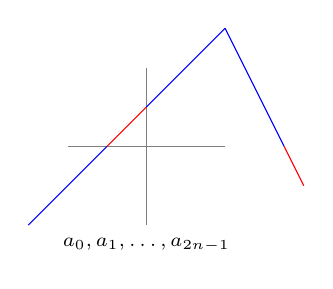
\begin{tikzpicture}[scale=0.5]
\draw[gray] (-2,0) -- (2,0);
\draw[gray] (0,-2) -- (0,2);
\draw[blue] (-3,-2) -- (-1,0);
\draw[red]  (-1,0) -- (0,1);
\draw[blue] (0,1) -- (2,3);
\draw[blue] (2,3) -- (3.5,0);
\draw[red]  (3.5,0) -- (4,-1);
\node at (0,-2.5) {\scriptsize $a_{0},a_{1},\ldots,a_{2n-1}$};
\end{tikzpicture}
}
\subfigure[Après le split]
{
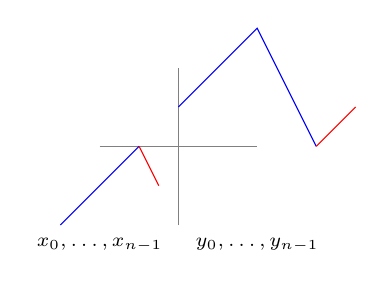
\begin{tikzpicture}[scale=0.5]
\draw[gray] (-2,0) -- (2,0);
\draw[gray] (0,-2) -- (0,2);
\draw[blue] (-3,-2) -- (-1,0);
\draw[red]  (-1,0) -- (-0.5,-1);
\draw[blue] (0,1) -- (2,3) -- (3.5,0);
\draw[red]  (3.5,0) -- (4.5,1);
\node at (-2,-2.5) {\scriptsize $x_{0},\ldots,x_{n-1}$};
\node at (2,-2.5) {\scriptsize $y_{0},\ldots,y_{n-1}$};
\end{tikzpicture}
}
\end{center}
\caption{Exemple de split bitonique}
\end{figure}

\subsection{Tri d'une suite bitonique}

Soit une suite bitonique de $n$ éléments. Si on applique le théorème
récursivement :
\begin{center}
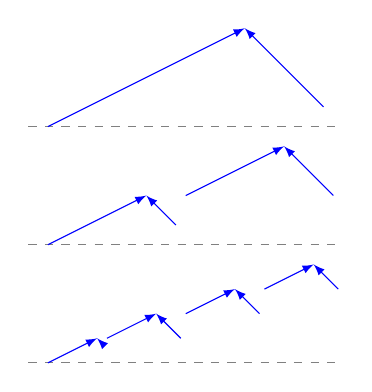
\begin{tikzpicture}[scale = 0.5]
\draw[dashed,gray] (0,0) -- (8,0);
\draw[blue,-latex] (0.5,0) -- (5.5,2.5);
\draw[blue,-latex] (7.5,0.5) -- (5.5,2.5);

\draw[dashed,gray] (0,-3) -- (8,-3);
\draw[blue,-latex] (0.5,-3) -- (3,1.25-3);
\draw[blue,-latex] (3.75,0.5-3) -- (3,1.25-3);
\draw[blue,-latex] (4,1.25-3) -- (6.5,2.5-3);
\draw[blue,-latex] (7.75,1.25-3) -- (6.5,2.5-3);

\draw[dashed,gray] (0,-6) -- (8,-6);
\draw[blue,-latex] (0.5,-6) -- (1.75,0.625-6);
\draw[blue,-latex] (1.875,0.5-6) -- (1.75,0.625-6);

\draw[blue,-latex] (2.,0.625-6) -- (3.25,1.25-6);
\draw[blue,-latex] (3.875,0.625-6)--(3.25,1.25-6);

\draw[blue,-latex] (4,1.25-6) -- (5.25,1.875-6);
\draw[blue,-latex] (5.875,1.25-6)--(5.25,1.875-6);

\draw[blue,-latex] (6,1.875-6) -- (7.25,2.5-6);
\draw[blue,-latex] (7.875,1.875-6)--(7.25,2.5-6);

\end{tikzpicture}
\end{center}

Après $\log(n-1)$ pas, chaque suite bitonique possédera seulement
deux éléments qui pourront être triés trivialement.

L'algorithme complet de tri consistera donc à :
\begin{enumerate}
\item Trier les $\frac{n}{2}$ premiers éléments dans l'ordre croissant et les
derniers $\frac{n}{2}$ éléments dans l'ordre décroissant
\item Trier la suite bitonique résultante en $\log{n}$ étapes.
\end{enumerate}

\textcolor{red}{Comment trier $\frac{n}{2}$ éléments ?} {\Large\textcolor{blue}{$\Rightarrow$}} \textcolor{red}{Récursivement}

La complexité de l'algorithme de tri est de :
\begin{itemize}
\item $\log(n)$ étapes;
\item Chaque pas $i$ demande $i$ sous-pas
\end{itemize}
Donc le nombre de pas est donc :
\[
\mbox{Nombre de pas} = \sum_{i=1}^{log(n)} i = \frac{1+\log(n)}{2}log(n)
\]

\subsection{Travail à faire}

Utiliser la version du tri fourni en séquentiel pour trier un tableau d'entier
puis un tableau de vecteurs selon leurs normes L2.

Paralléliser à l'aide des threads de C++ 2011 l'algorithme de tri puis calculer
l'accélération obtenue pour le tri sur les entiers puis pour le tri sur les vecteurs.

Comment interprétez-vous la différence d'accélération entre le tri sur les entiers et
le tri  sur les vecteurs ?

\section{Ensemble de Bhudda}

L'ensemble de bhudda est un ensemble dérivé de l'ensemble de Mandelbrot. Au lieu de dessiner des pixels en fonction
du nombre d'itérations nécessaires à la détection éventuelle de divergence de la suite, on augmente l'intensité de chaque
pixel par lesquels une suite divergente est passée ( on ne fait rien pour les suites convergentes ).
\`A l'aide d'OpenMP, paralléliser le code Bhudda donné dans le fichier \texttt{bhudda.cpp}

\end{document}
